\documentclass{article}


% if you need to pass options to natbib, use, e.g.:
%     \PassOptionsToPackage{numbers, compress}{natbib}
% before loading neurips_2024


% ready for submission
\usepackage{neurips_2024}


% to compile a preprint version, e.g., for submission to arXiv, add add the
% [preprint] option:
%     \usepackage[preprint]{neurips_2024}


% to compile a camera-ready version, add the [final] option, e.g.:
%     \usepackage[final]{neurips_2024}


% to avoid loading the natbib package, add option nonatbib:
%    \usepackage[nonatbib]{neurips_2024}

\usepackage{graphicx} 
\usepackage[utf8]{inputenc} % allow utf-8 input
\usepackage[T1]{fontenc}    % use 8-bit T1 fonts
\usepackage{hyperref}       % hyperlinks
\usepackage{url}            % simple URL typesetting
\usepackage{booktabs}       % professional-quality tables
\usepackage{amsfonts}       % blackboard math symbols
\usepackage{nicefrac}       % compact symbols for 1/2, etc.
\usepackage{microtype}      % microtypography
\usepackage{xcolor}         % colors

\usepackage{biblatex} %Imports biblatex package
\addbibresource{bibliography.bib} %Import the bibliography file

\title{Semiconductor Layout Design with Large Language Models: Opportunities and Challenges}

\author{%
  Bo Wen\\
  IBM Watson Research Center, \\
  Yorktown Heights, NY, USA \\
  \texttt{bwen@us.ibm.com} \\
  \And
  Xin Zhang\\
  IBM Watson Research Center, \\
  Yorktown Heights, NY, USA \\
  \texttt{xzhang@us.ibm.com} \\
}

\begin{document}

\maketitle

\begin{abstract}
  % Update abstract to reflect the content of the paper
  This paper explores the potential of large language models (LLMs) as a "layout design copilot" in various domains such as semiconductor, IC, and microfluidics. We evaluate the capabilities of LLMs in generating basic elements and combining them into complex designs. Our experiments focus on via connections, microfluidics channel design, and fiducial marker generation. We discuss the opportunities and challenges of using LLMs in layout design, highlighting the importance of providing expert knowledge and context to improve their performance.
\end{abstract}

\section{Introduction}
The semiconductor industry faces significant challenges in layout design, a critical step in the development of integrated circuits (ICs), microfluidic chips, and other electronic devices. A key issue is the limited adaptability of current graphical user interface (GUI) based design workflows to diverse application needs. This inflexibility often results in inefficient, repetitive tasks of creating similar structures with minor variations, such as many copies of similar serpentine patterns in microfluidic chips which only differ in width, length, number of turns, and turning radii. This approach not only violates the "Don't Repeat Yourself" (DRY) principle of software development but also leads to potential inconsistencies and reduced productivity in the design process.

Traditional layout design software, primarily relying on GUI-based interactions rather than scripting languages, has struggled to address these adaptability challenges effectively. However, the emergence of Large Language Models (LLMs) presents a promising opportunity to revolutionize the layout design process. LLMs have demonstrated remarkable capabilities in understanding natural language instructions and generating code, making them ideal candidates for creating a "layout design copilot." We can envision a new paradigm of design workflow where human designers provide high-level design intent and the copilot generates the layout code, with the designer playing a more supervisory role and spending more time on high-level tasks that require creativity and intuition.

In this paper, we explore the capabilities and limitations of state-of-the-art Large Language Models (LLMs) in semiconductor layout design tasks. Our main contributions are:

1. Establishing a baseline performance of five state-of-the-art LLMs on 25 common layout design tasks, evaluating their zero-shot capabilities (Section 2).

2. Analyzing the mistakes made by these LLMs and categorizing common errors in layout design tasks. Our analysis indicates that some of these errors can be addressed by Retrieval-Augmented Generation (RAG) and In-Context Learning (Section 2).

3. Documenting an iterative design process of multimodal inputs with GPT-4o for a complex task (ViaConnection), illustrating the limitations of current LLMs in spatial reasoning (Section 3).

4. Introducing a novel Neuro-inspired LLM Reasoning Network architecture that leverages multiple LLMs to improve reasoning capabilities and mitigate hallucinations in layout design tasks (Section 4).

5. Presenting preliminary results demonstrating the effectiveness of our proposed architecture compared to single-LLM baselines (Section 4).

Finally, Section 5 concludes the paper and discusses future research directions.

\section{Baseline LLM Performance in Layout Design}

We evaluated the performance of five large language models (LLMs) - GPT-4o, Claude-3.5-Sonnet, Llama-3.1-70B, Llama-3.1-405B and the new ``reasoning model'', o1-preview - on a set of 25 layout design tasks. Each tasks have been run 5 times with same prompt and temperature = 0.7. We then run the LLM written code to generate a GDSII file and further convert the GDSII to png images for human evaluation. These tasks were categorized into four groups: Basic Shapes 1, Basic Shapes 2, Advanced Shapes, and Complex Structures. Figure \ref{fig:baseline-llm-performance} presents a summary of the LLMs' performance across the task categories. See Appendix for the task prompts and detailed results.

\begin{figure}[h]
  \centering
  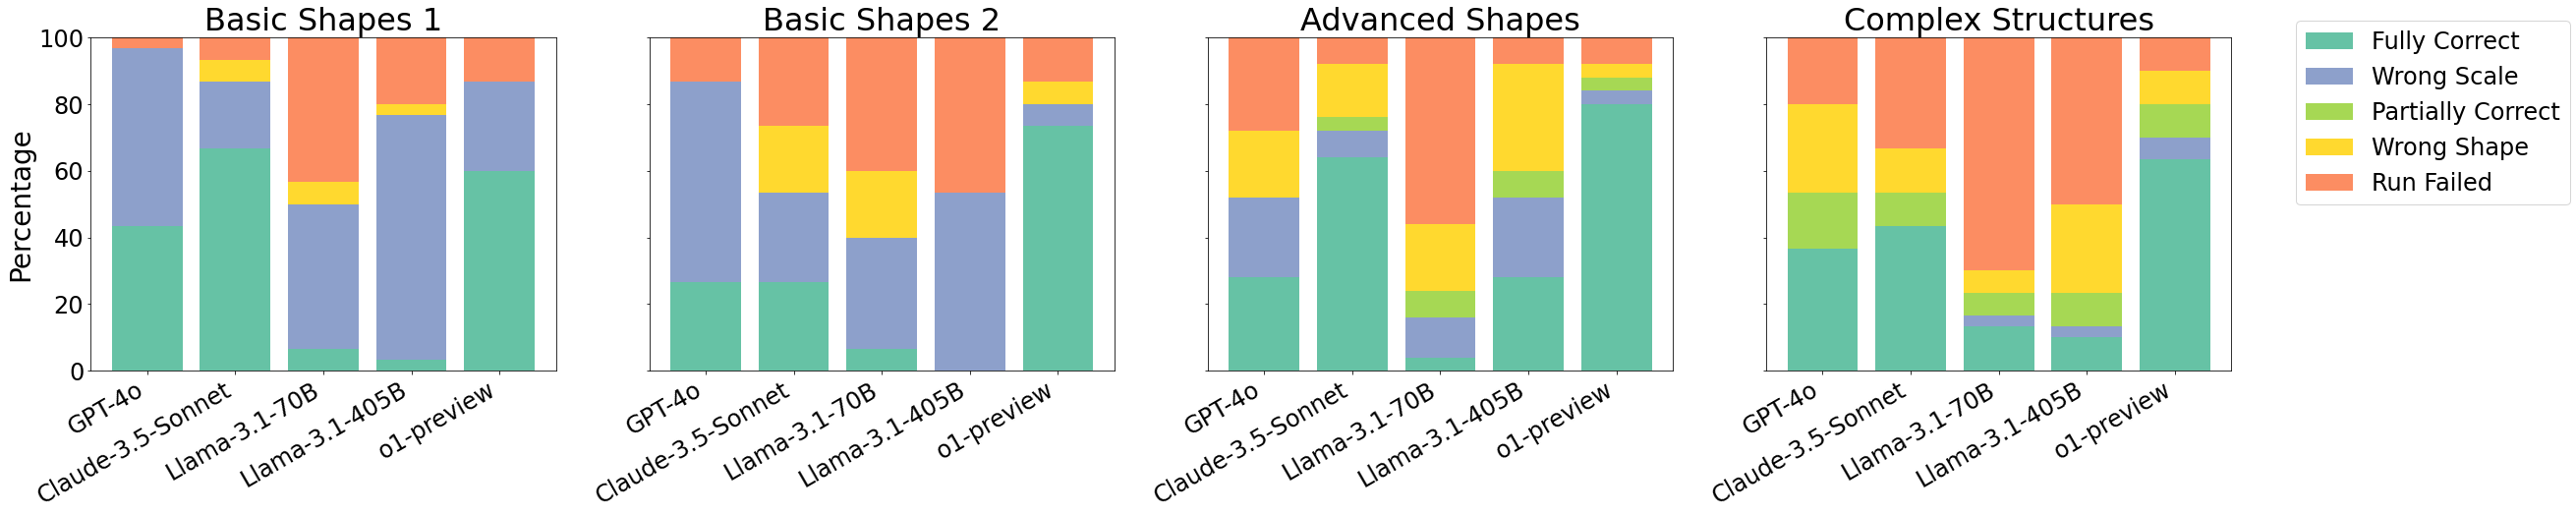
\includegraphics[width=\textwidth]{baseline-llm-performance.png}
  \caption{Baseline LLM Performance on Layout Design Tasks}
  \label{fig:baseline-llm-performance}
\end{figure}

The results reveal several common mistakes and limitations of standalone LLMs in handling layout design tasks:

\begin{enumerate}
  \item \textbf{Incorrect scaling}: The default unit in the gdspy library is micrometers. But we requested the basic shapes to be drawn in millimeters, in order to test whether the LLM could correctly figure out this catch and scale the shapes according to the specified units. As can be seen from the dark blue ``Wrong Scale'' part of bar chart, all the LLMs struggled to various degrees: (a) Sometimes the LLMs simply failed to pay attention to the requested unit (millimeters) and did not perform the necessary scaling. (b) In some cases, LLMs did pay attention to the requested unit but made incorrect assumptions about gdspy's default unit. We observed many hallucinations of millimeters and resulting in no scaling. Interestingly, we observed one case where Claude-3.5-Sonnet hallucinated that the default unit was nanometers, leading it to scale the length by 1e6. This resulted in shapes too large to be drawn. (c) From the chart, we can see that Llama-3 models are especially vulnerable to this issue. They sometimes even assumed the user had made a mistake by requesting millimeters, and proceeded to draw in micrometers instead, justifying this choice with comments like "not mm, as the GDSII format is in micrometers". This type of ``arrogant'' behavior and misalignment with human instructions on simple tasks will be very harmful for deploying LLMs as fully automanous AI agents. A recent Nature paper \cite{ZhouNature2024} has also discussed similar observations.
  
  \item \textbf{Partial correctness}: In more complex tasks, LLMs often generated partially correct layouts with mistakes in the relative positioning of simple shapes. For example, in the ViaConnection task, which involved specific relative location requirements like ``Ensure the metal connection fully covers the vias and leaves a margin of 10 units between the edge of the metal and the pads. Leave a space of 50 units between the vias and the edges of the metal connection.'', only o1-preview achieved one fully correct result. The other LLMs all produced partially correct outputs as shown in the yellow ``Partially Correct'' part of the bar chart.
  
  \item \textbf{Runtime errors}: Approximately one third of the generated code from the evaluated LLMs resulted in exceptions and failed to execute. The most frequent error, \textit{AttributeError: module 'gdspy' has no attribute 'LayoutViewer'}, occurred 26 times (59.09\%) with GPT-4o and 33 times (61.11\%) with Claude-3.5-Sonnet. In contrast, this error was reported only once each for Llama-3.1-70B and o1-preview, and not at all for Llama-3.1-405B, indicating that GPT-4o and Claude-3.5-Sonnet are trying to be more ``helpful'' by providing GUI output, which is not available in the runtime environment. This is not entirely LLM's fault, but due to missing information in the prompt. The second most common errors were due to hallucinations of nonexistent `gdspy` functions or methods, including various `AttributeErrors` (e.g., `'CrossSection'`, `'Circular'`, `'Ellipse'`) and `TypeErrors`. This also includes spelling error, for example, miss spelling \textit{gdspy.Text} as \textit{gdspy.text}. Additionally, other frequent issues involved typical programming logic mistakes such as missing module imports or incorrect function parameters. For more details, see the error report in (Appendix).
  
  \item \textbf{Inefficient code}: There's one special case that we'd like to point out. In the DLDChip task, which involves creating a dense array of identical shapes, the Llama-3.1-405B model generated a code that created a large number of objects and performed numerous boolean operations, leading to high memory usage and extended execution time. We have to kill the code after about 15 mins of waiting. 
\end{enumerate}

These findings highlight the limitations of standalone LLMs in handling complex layout design tasks. While they perform relatively well on basic shapes, their performance deteriorates as the task complexity increases. The common mistakes and inefficiencies underscore the need for a more advanced approach to tackle these challenges effectively.

A total of 25 examples were generated using ChatGPT-4o, Python code was generated to write a GDSII files for the desired elements, accompanied by human evaluation. In instances where the model did not produce the correct output on the first attempt, a researcher would provide step-by-step guidance until achieving the desired result. However, in the case of generating a serpentine pattern, the model encountered difficulties, likely due to an unfamiliarity with the \texttt{gdspy.FlexPath} function. To address this, an example code was provided to the model, enabling it to 'learn' and successfully generate the correct serpentine sample file.

\subsection{Via Connection Experiment}
\subsubsection{Background}
In semiconductor processes, vias are essential for creating electrical connections between different layers of a chip. Proper via placement and connection are crucial for ensuring the functionality and reliability of the integrated circuit. This experiment explores the potential of using large language models (LLMs) to generate layout designs for via connections based on natural language descriptions and color-coded sketches.
\subsubsection{Experimental Setup}
The sketch-to-design approach using LLMs involves providing a natural language description of the desired via connection layout along with a color-coded sketch. The input format consists of a text description specifying the layers, dimensions, positions, and connectivity requirements, as well as a corresponding sketch where each color represents a specific layer (e.g., yellow for via, blue for metal, red for pad). The target output is Python code that generates the GDSII layout based on the provided description and sketch.
\subsubsection{Iterative Testing and Results}
We conducted a series of tests to evaluate the LLM's performance in generating via connection layouts. Figure \ref{fig:via_experiment} presents the sketch input and the corresponding outputs generated by the LLM for each test case.
\begin{figure}[!h]
\centering
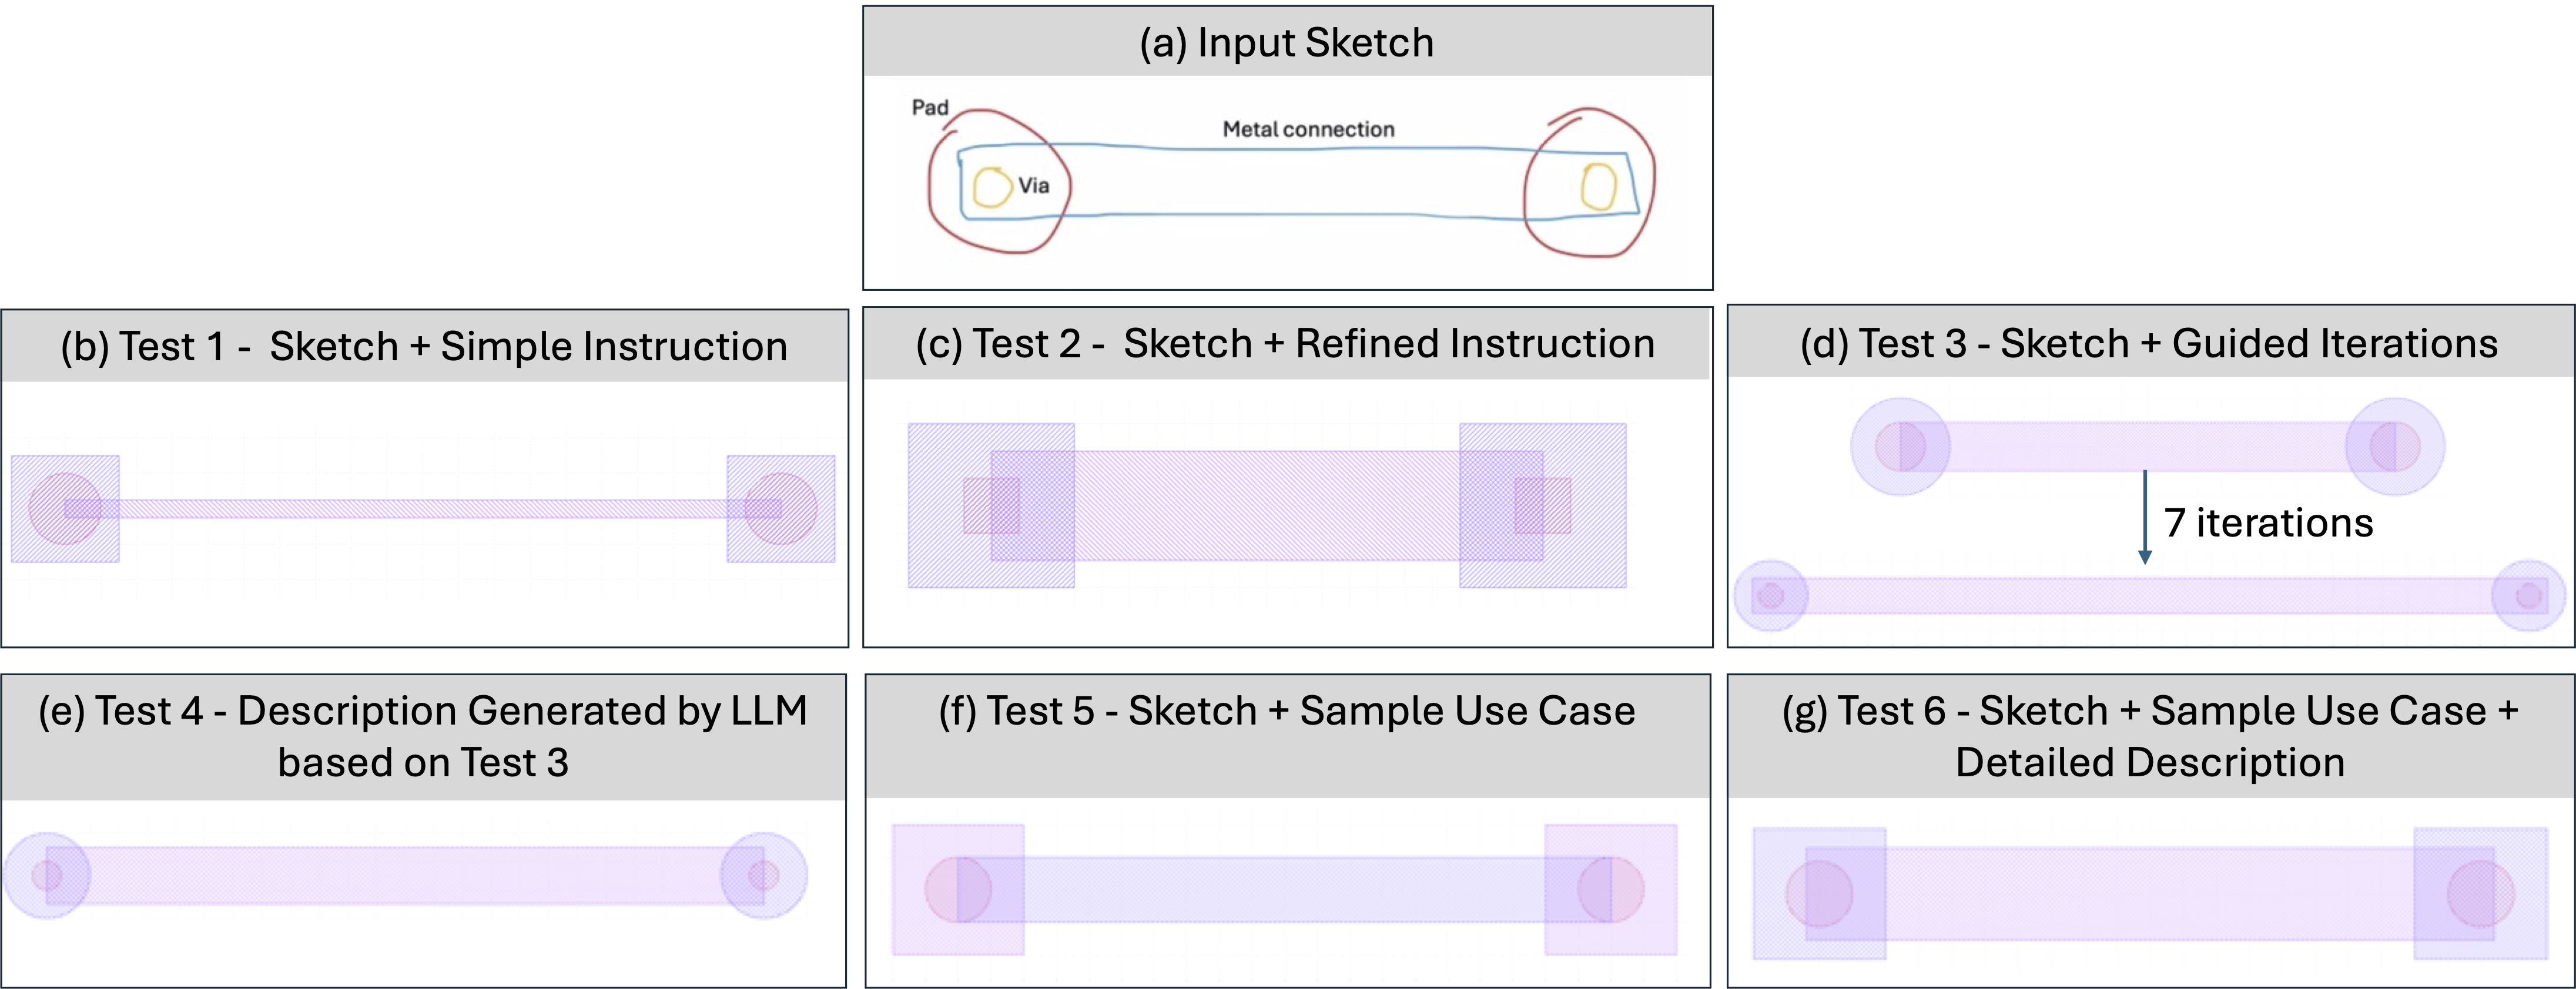
\includegraphics[width=1\linewidth]{Figure1_v3.png}
\caption{Sketch input and LLM-generated outputs for the via connection experiment. The sketch depicts a desired layout with two vias connected by a metal layer and circular pads on top. The outputs show the progression of the LLM's understanding and refinement of the layout based on iterative feedback and context provided by the user.}
\label{fig:via_experiment}
\end{figure}
In \textbf{Test 1}, we provided a basic sketch (Figure ~\ref{fig:via_experiment}(a)) along with a simple instructions to inform it each color represented a different layer. The LLM generated code based on this initial description; however, the output presented several issues, including incorrect dimensions for various elements and inaccurate layer relationships. \textbf{Test 2} involved refining the description, but limited improvement is observed. 

In \textbf{Test 3}, we gave a more detailed description accompanied by the original sketch. We proceeded with an iterative process, providing the LLM with feedback and screenshots of the GDSII file generated from its code. After seven iterations, the LLM successfully produced the correct layout. \textbf{Test 4} aimed to reproduce the best output from the previous test. We requested the LLM to create a detailed prompt based on the successful result from Test 3 and used this prompt to attempt to generate the correct output again. However, this approach proved ineffective, indicating that relying solely on an LLM-generated prompt to reproduce a layout was not reliable.

\textbf{Tests 5} and \textbf{6} gradually incorporated more context, such as 3D packaging, Through-Silicon Vias (TSVs), and other domain-specific requirements. However, adding domain knowledge and context did not improve the LLM's performance much, showcasing both its limitations and areas for potential improvement. Experienced engineers and researchers understand that connecting two vias requires using a metal layer wider than the diameter of the via. Moreover, vias should not be placed at the very ends of metal layers; some leeway is typically be left between layers to accommodate potential misalignment.

The experiments demonstrate that LLMs currently lack the domain-specific knowledge possessed by experienced engineers, such as the need for wider metal connections between vias and leeway for misalignment. Despite incorporating more context and domain requirements in\textbf{Tests 5} and \textbf{6}, improvements were minimal, highlighting the gap in the LLM's understanding. Future development should focus on embedding domain-specific rules and enhancing consistency and reproducibility.



\subsubsection{Lessons Learned}
The via connection experiment revealed several key findings:
\begin{itemize}
\item Clear, detailed, and context-rich input is essential for LLMs to generate accurate layout designs.
\item Iterative refinement and user feedback play a crucial role in guiding the LLM towards the desired output.
\item LLMs have limitations in understanding domain-specific requirements and constraints without explicit guidance.
\end{itemize}
\subsubsection{Potential Improvements and Future Work}
To enhance the sketch-to-design approach for via connections, we propose incorporating domain-specific knowledge and design rules into the LLM prompts. This can be achieved by providing a comprehensive set of guidelines and constraints as part of the input description. Additionally, future experiments should focus on validating the effectiveness of the improved approach and exploring its applicability to more complex via connection scenarios.

\section{Neuro-inspired LLM Reasoning Network Architecture}

In this section, we present a novel Neuro-inspired LLM Reasoning Network Architecture designed to enhance the reasoning capabilities of large language models (LLMs) and mitigate the issue of hallucinations in generated outputs. This architecture is particularly well-suited for complex domains such as semiconductor layout design, where the ability to generate accurate and consistent results is critical.

The proposed architecture is inspired by the Brain-like AGI and the Free Energy Principle (FEP) theory. It consists of three main components: Thought Generator Pool, Thought Assessors, and a Steering Subsystem. The Thought Generator Pool is a multi-LLM network that generates initial attempts at a given task by exploring different approaches and perspectives. This multi-LLM approach allows for a more comprehensive exploration of the problem space compared to traditional single-model approaches. It is effectively a Tree-of-Thoughts combined with parallel searching. Because different LLMs have distinct pre-train data and architecture and embedding spaces, this approach can effectively sample diverse solutions from human knowledge space.

The Thought Assessors, also implemented as LLMs, evaluate the outputs generated by the Thought Generator Pool. They analyze the initial attempts, identify consistencies and discrepancies, and reach a consensus on the most promising solutions. By examining the differences between the initial outputs, the Thought Assessors can identify potential hallucinations and mistakes, enabling the system to produce more robust and accurate results.

In the current implementation, a human serves as the Steering Subsystem, coordinating interactions and guiding the overall reasoning process. Additionally, the human performs the active inference function within the Free Energy Principle (FEP) framework. In future work, we aim to develop an automated Steering Subsystem that can distill the system's successes and failures into its knowledge base (a Retrieval-Augmented Generation (RAG) database) to support continual learning.

One of the key advantages of this architecture is its ability to facilitate personal and domain adaptation. By leveraging RAG and continual learning, the system can effectively adapt to specific users' preferences and domain-specific knowledge. This adaptability is particularly valuable in the context of semiconductor layout design, where the ability to tailor the system's outputs to individual designers' needs and domain-specific constraints is essential.

figure 1

Figure 1 illustrates the high-level architecture of the Neuro-inspired LLM Reasoning Network. The Thought Generator, consisting of multiple LLMs, generates initial attempts at the given task. The Thought Assessors evaluate these attempts, identify discrepancies, and reach a consensus on the most promising solutions. The Steering Subsystem coordinates the interactions between the Thought Generator and Thought Assessors, incorporating techniques like RAG and continual learning to enhance the system's adaptability.

figure 2

Figure 2 provides a more detailed view of the interaction between the Thought Generator and Thought Assessors. The Thought Generator produces multiple initial attempts, which are then evaluated by the Thought Assessors. The assessors identify consistencies and discrepancies among the attempts, enabling the detection of potential hallucinations and mistakes. This process allows the system to generate more robust and accurate outputs.

The proposed Neuro-inspired LLM Reasoning Network Architecture offers a significant improvement over traditional single-model approaches in terms of zero-shot accuracy and the ability to avoid hallucination-induced mistakes. By leveraging the power of multiple LLMs and incorporating techniques like RAG and continual learning, this architecture enables more effective reasoning and adaptability in complex domains such as semiconductor layout design.

\section{Conclusion and Future Work}
% Recap the main findings and insights
% Discuss the potential of LLMs in layout design and the challenges to overcome
% Outline future research directions:
%   - Dealing with more complicated designs
%   - Creating a benchmark to test LLM capabilities in layout design tasks
% Final thoughts on the role of LLMs as a "layout design copilot"
agent \cite{Ho2024-cd}
other domains, like mechanics, architecture (3d virtual space \cite{Sasazawa2024-wf})

% \printbibliography %Prints bibliography

\end{document}